\documentclass[tikz,border=2pt]{standalone}
\usepackage{amsmath,amssymb}
\usepackage{tikz}

\begin{document}
% Two fair dice and g(x, y) = 1{x + y = 7}: LOTUS sums g times the joint mass over all 36 pairs;
% only the six pairs on the anti-diagonal contribute.
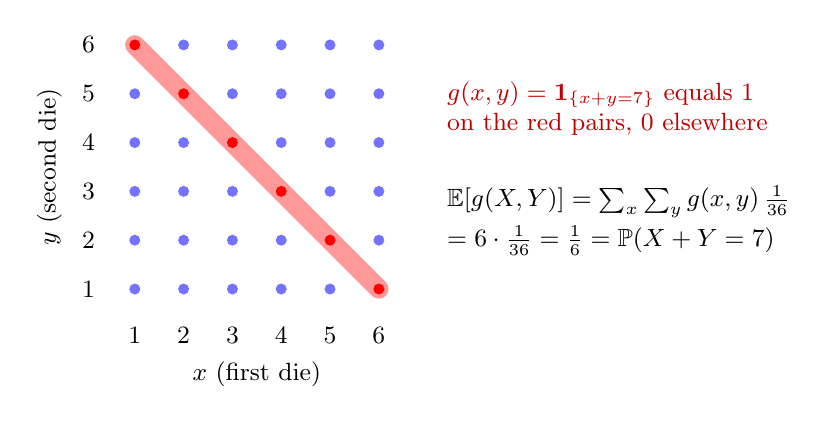
\begin{tikzpicture}[every node/.style={font=\small}, scale=0.62]
	\draw[red!40, line width=7pt, line cap=round] (1,6) -- (6,1);
	\foreach \x in {1,...,6} {
		\foreach \y in {1,...,6} {
			\pgfmathtruncatemacro{\s}{\x+\y}
			\ifnum\s=7
				\fill[red] (\x,\y) circle (3.2pt);
			\else
				\fill[blue!55] (\x,\y) circle (3.2pt);
			\fi
		}
		\node[font=\small] at (\x,0.05) {$\x$};
		\node[font=\small] at (0.05,\x) {$\x$};
	}
	\node[font=\small] at (3.5,-0.75) {$x$ (first die)};
	\node[font=\small, rotate=90] at (-0.75,3.5) {$y$ (second die)};
	\node[red!75!black, anchor=west, align=left] at (7.2,4.7) {$g(x,y)=\mathbf{1}_{\{x+y=7\}}$ equals $1$\\ on the red pairs, $0$ elsewhere};
	\node[anchor=west, align=left] at (7.2,2.4) {$\mathbb{E}[g(X,Y)]=\sum_x\sum_yg(x,y)\,\tfrac1{36}$\\[2pt] $=6\cdot\tfrac1{36}=\tfrac16=\mathbb{P}(X+Y=7)$};
	
\end{tikzpicture}
\end{document}
